% !TeX root = ../../thesis.tex

\section{\acf{UEFI}}

The \ac{UEFI} specification is a pure interface specification, describing a programmatic interface for boot applications to interact with the \ac{PF}.
It states what interfaces, structures, and abstractions a \ac{PF} has to offer and implement and what boot applications such as \ac{OS} loaders may use \cite{beyond-bios}.

It was designed to replace the legacy \acl{BF} \ac{BIOS}, while also providing backwards compatibility with a \acf{CSM} allowing \ac{UEFI} firmware to boot legacy \ac{BIOS} applications \cite{beyond-bios}.
It is aimed to be a complete solution, abstracting all platform features and capabilities in a way that bootloaders require no knowledge about the underlying hardware \cite[1.3]{uefi-spec}.

The \ac{UEFI} interfaces are defined in the \code{C} programming language.
During the boot process, system resources are owned and managed by the \ac{UEFI} firmware until the \ac{OS} explicitly assumes control over the system.
On the \code{x64} \ac{CPU} architecture the \ac{PF} hands over execution in \code{64-bit} long mode which includes memory protection.
Paging is also enabled and the virtual memory is identify mapped, meaning virtual addresses equal physical addresses, while most regions are read, write, and execute.
The \ac{CPU} is operating in uniprocessor mode and a sufficient amount of stack is available \cite[Section 2.3.4]{uefi-spec}.

Since \ac{UEFI} mainly exists to offer a well\-/defined boot environment for \ac{OS} loaders, its services are not required anymore upon \ac{OS} takeover.
A large part of \ac{UEFI} can thus be unloaded, leaving only a portion of the initially offered services.
The remaining runtime services can be used by the \ac{OS} to configure or update the \ac{PF}.

\subsection{\acf{GUID}}

The \ac{UEFI} environment depends on \acp{GUID}, also known as \acp{UUID}, to uniquely identify a variety of things, such as protocols, files, and hard drive partitions.
\acp{GUID} are 128-bit long, statistically unique identifiers that can be generated on demand and without a centralized authority, statistically guaranteeing that there will be no duplicates on a system that combines hard- and software from multiple vendors \cite{rfc-4122}.

\subsection{\acf{GPT}}

Partitions allow a disk to be distinctly separated into logical disks, allowing for each to be formatted with a different file systems.
Prior to \ac{UEFI} disks have been partitioned using the \ac{MBR} partition table, supporting up to four different partitions.
The \ac{MBR} is stored within the first sector, also optionally containing 424 bytes of bootable code through which the \ac{BIOS} boots \cite[Section 13.3.1]{uefi-spec}.
\ac{UEFI} is still backwards compatible with \ac{MBR} partitioned disks and contained on each disk, but \ac{UEFI} does not execute the boot code.
The \ac{MBR} is used in two different ways by the \ac{UEFI} environment, either as a legacy \ac{MBR} or a protective \ac{MBR}.
With the legacy \ac{MBR}, \ac{UEFI} uses the partitions defined in the \ac{MBR} partition table, whereas the protective \ac{MBR} only has one partition spanning the entire disk.
The protective partition is for legacy devices and, in practice, \ac{GPT} partitioning is used to separate the disk.
For this, \ac{UEFI} defines two \ac{OS} types used in \ac{MBR} partition entries.
One identifies the \ac{ESP}, the partition \ac{UEFI} boots from, within the legacy \ac{MBR} partition table and the other indicates that a protective partition is used \cite[Section 5]{uefi-spec}.
\cite[Section 5]{uefi-spec} defines the \ac{GPT} disk layout. With the \ac{GPT} format, \ac{LBA} are 64-bit instead of 32-bit, enabling support for drives with up to 9400000000 \ac{TB} of storage, whereas \ac{MBR} is limited to 2 \ac{TB}.
This is accompanied by allowing more than four partitions, with Windows supporting up to 128 \cite{microsoft-windows-and-gpt-faq}.
\acp{GUID} are used to identify partitions and partition types, but also offering a human readable partition name.
\ac{GPT} also has a primary and a backup partition table for redundancy purposes.
The primary table follows the \ac{MBR} sector and the backup is at the end of the disk.

\subsection{\acf{ESP}}

The \ac{ESP} can reside on any media that is supported by the \ac{UEFI} firmware.
It has to be formatted in \ac{FAT}32 \cite[Section 13.3]{uefi-spec} and must contain an \program{EFI} root directory \cite[Section 13.3.1.3]{uefi-spec}.
All \ac{UEFI} applications that are to be launched directly by the \ac{UEFI} firmware have to be located in sub\-/directories below the \program{EFI} directory \cite[Section 13.3.1.3]{uefi-spec}.
Drivers and indirectly loaded applications have no storage restrictions.
Vendors are to use vendor\-/specifically named sub\-/directories within the \program{EFI} directory.
Fixed disks have no restrictions on the amount of \acp{ESP} present, whereas removable media is only allowed to have one \ac{ESP}, so that boot behavior is deterministic.
In general, the \ac{ESP} is identified by a specific \ac{GUID}, but implementations are allowed to support accordingly structured \ac{FAT} partitions.
Since there is no limitation on the amount of \acp{ESP}, boot applications can share the drive with their \ac{OS}, or can be accumulated in a single system\-/wide \ac{ESP} \cite[Section 13.3.3]{uefi-spec}.

\subsection{\acs{UEFI} Images}

\ac{UEFI} images are files containing executable code. They use a subset of the \ac{PE32}+ file format with a modified header signature.
The format comes with relocation tables, making it possible for the images to be executed in place or to be loaded at non-pre\-/determined memory addresses.
They support multiple CPU architectures such as IA, ARM, RISC-V, and x86.
There are three different subtypes of executables: applications, boot, and runtime drivers. They mainly differ in their memory type and how it behaves.
Loading and transferring execution are two separate steps, so that security policies can be applied before executing a loaded image \cite[Section 2.1.1]{uefi-spec}.

Applications are always unloaded when they return from execution, while drivers are only unloaded when they return an error code. This allows drivers to install their offered functionality upon initial execution and function calls can jump back into the driver image where the function body remains loaded.
Boot drivers are unloaded when an \ac{OS} loader application transitions to runtime by taking over the memory management through the call of the boot service function \code{ExitBootServices()}, while runtime drivers remain loaded and are translated into the virtual memory mapping. \ac{OS} loaders only return execution in error cases.

\subsection{Protocols and Handles}

Protocols are created and discovered dynamically and provide a mechanism to enable an extension of firmware capabilities over time \cite[Section 3.6]{tianocore-edk2-driver-writer-s-guide}.
They are C structures and may contain services, in the form of function pointers, or other data structures.
They are identified by \acp{GUID} and stored in a single global database implemented by the firmware \cite{beyond-bios}.
This database is called the handle database, handles describe a logical grouping of one or more protocols \cite[Section 3.6]{tianocore-edk2-driver-writer-s-guide}.
Handles are unique per session and should not be saved across reboots \cite{beyond-bios}.
Multiple instances of a protocol identified by the same \ac{GUID} can exist on different handles, offering the same service on different devices.

\begin{figure}[htb]%
    \centering%
    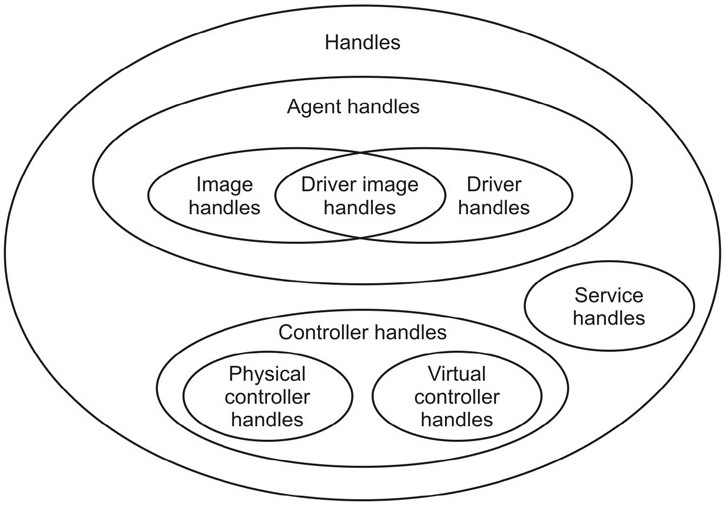
\includegraphics[width=0.7\textwidth]{uefi/handle_types}%
    \caption[Handle types]{Handle types (taken from \cite[Figure 3]{tianocore-edk2-driver-writer-s-guide})}%
    \label{fig:handle-types}%
\end{figure}

\cite{tianocore-edk2-driver-writer-s-guide} explains the categories of handles that are formed by the type of protocols that are grouped. \autoref{fig:handle-types} shows these categories.

\begin{description}
    \item[Image handles] are handles of \ac{UEFI} images loaded into memory, as they support the \hyperref[lst:loaded-image-protocol]{Loaded Image Protocol}, giving access to information about the image in memory. This includes the image's address, size, memory type, origin, and optional load options.
    \item[Driver handles] are handles that group the \ac{UEFI} Driver Model related protocols (Driver Binding Protocol, the two Component Name Protocols, and the two Driver Diagnostics Protocols).
    \item[Driver image handles] are \ac{UEFI} Driver Model related protocols installed onto images loaded in memory.
    \item[Agent handles] is a term used in the \ac{UEFI} Driver Model, they describe tracked consumers of other protocols.
    \item[Controller/Device handles] are interchangeably used to refer to physical and virtual devices that offer \ac{I/O} abstraction protocols.
        Physical device handles support the Device Path Protocol for generic path/location information \cite[Section 10.2]{uefi-spec}.
    \item[Service handles] are used for generic hardware unrelated abstractions.
\end{description}

\subsection{\acs{UEFI} Driver Model}

\cite[Section 2.5]{uefi-spec} describes the \acs{UEFI} Driver Model.
It is designed to simplify the implementation process of device drivers by moving common device management and discovery functionality into the firmware.
This leaves drivers with the responsibility to offer only interfaces for installation and removal.

An \ac{UEFI} platform is assumed to consist of one or more \acp{CPU} to be connected to one or more core chipsets.
The core chipsets produce host bus controllers which offer initial \ac{I/O} abstractions like the \ac{PCI} Root Bridge \ac{I/O} Protocol.
Bus drivers can be connected to these host bus controllers to discover and create child controllers, these can either be further buses or devices.
This forms a tree of buses with devices as leaves.
Devices can be keyboards, mice, monitors, etc. (for user in\-/and output) or hard drives, network adapters, etc. (boot devices) \cite[Section 2.5]{uefi-spec}.

Device drivers are very similar to bus drivers, but they do not create new device handles, they instead offer abstractions built upon existing bus driver \ac{I/O} abstractions.
A driver following the \ac{UEFI} Driver Model is not allowed to interact with any hardware in its entry point and instead installs protocols on its own image handle.
It is required to install the Driver Binding Protocol and it may additionally install configuration or diagnostic related protocols.
The Loaded Image Protocol also offers a field where a driver can provide a function through which it can be unloaded.
Runtime drivers usually register a notification function that is triggered when an \ac{OS} loader calls \code{ExitBootServices()}, allowing them to translate any allocated memory to their virtual addresses \cite[Section 2.5.2]{uefi-spec}.

The firmware will try to connect device drivers to a controller by using the drivers instance of the Driver Binding Protocol and call the \code{Supported()} function on a controller handle.
The device driver then checks whether it supports the controller.
This could be, for example, looking for specific \ac{I/O} protocols, that it will want to use later and abstract further.
If the driver supports the device, the firmware will call the \code{Start()} function of the Driver Binding Protocol to have the driver install its offered protocols on the controller handle.
The firmware connection process can be done recursively as the newly installed device driver might now fulfill the requirements for another driver.
If a driver needs to be uninstalled from a specific controller, the firmware can call the \code{Stop()} method of the Driver Binding Protocol function on the controller handle.
An example for this would be another device driver wanting to exclusively manage a controller.
To support this functionality, all consumers of a protocol are tracked in the form of agent handles \cite[Section 2.5.4]{uefi-spec}.

The part of the firmware that will connect the device drivers is typically the \ac{UEFI} boot manager.
This allows for fast startup, where it may choose to connect only drivers related to a certain boot device \cite[Section 2.5.6]{uefi-spec}.

\subsection{Systemtable}

\lstinputlisting[language=C,caption={\acs{UEFI} Image Entry Point},captionpos=b,label=lst:entry-point]{code/entry_point.c}

\autoref{lst:entry-point} shows the entry point of \ac{UEFI} images, when they are loaded it is the only part that is \emph{linked}, the rest of the communication has to be discovered programmatically through the \ac{UEFI} System Table.
It serves as the entrance door into the \ac{UEFI} environment, providing access to the generic boot and runtime services, as well as system configuration information \cite[Section 3.3]{tianocore-edk2-driver-writer-s-guide}.
The Loaded Image Protocol instance provides an interface to hand over optional load options to an image \cite{beyond-bios}.

\autoref{fig:uefi-system-table} shows the system table.
The functionality of the system table is only available in its entirety during boot as the boot services and structures are eventually unloaded, when the \ac{OS} takes over control.

\begin{figure}[htb]%
    \centering%
    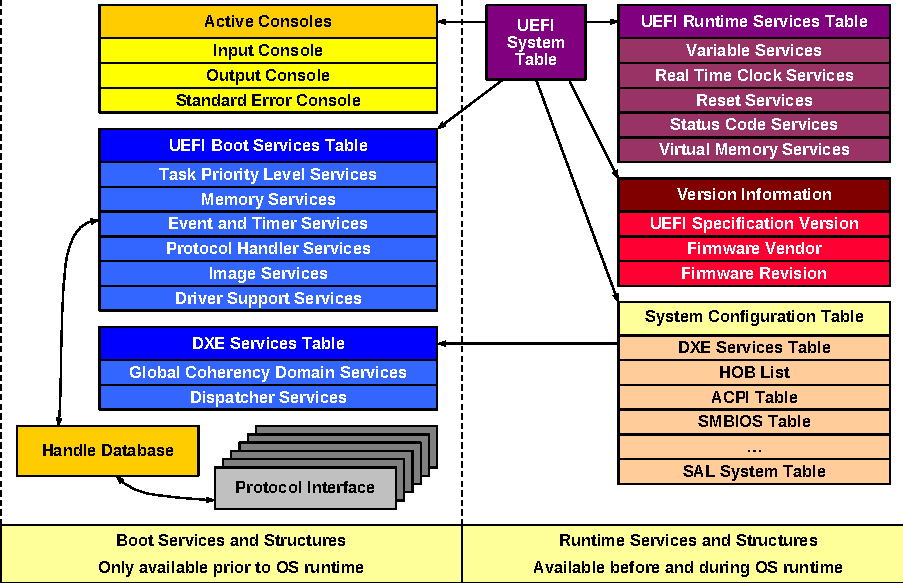
\includegraphics[width=0.8\textwidth]{uefi/uefi_system_table}%
    \caption[\acs{UEFI} System Table]{\acs{UEFI} System Table (taken from \cite[Vol 2, Figure 2-5]{pi-spec})}%
    \label{fig:uefi-system-table}%
\end{figure}

\subsubsection{Boot Services}

\ac{UEFI} applications must use boot service functions to access devices and allocate memory.
They are available until an \ac{OS} loader takes over control with \code{ExitBootServices()}.
\cite[Section 7]{uefi-spec} splits the boot services into five categories:

\begin{description}
    \item [Event, Timer, and Task Priority Services] used to create, close, signal, wait for, and check events. Setting timers and raising or restoring task priority levels.
    \item [Memory Allocation Services] to allocate and free pools or whole pages of memory, as well as retrieve the \ac{UEFI} managed memory map.
    \item [Protocol Handler Services] used to install, uninstall, and retrieve protocol instance as well as abstractions related to the \ac{UEFI} Driver Model.
    \item [Image Services] to load, unload, and start images. Images can also use these to transfer execution back to the firmware or with \code{ExitBootServices()} assume control over the system
    \item [Miscellaneous Services] offer basic memory manipulation, checksum calculation, watchdog timers, and monotonic counters.
\end{description}

\subsubsection{Runtime Services}

The runtime services only offer minimal functionality for the \ac{OS} to communicate with the \ac{PF} during runtime.

\begin{description}
    \item [Variable Services] used to query, get, and set \hyperref[sec:uefi-pi:uefi:variables]{variables}.
    \item [Time Services] used to get and set time as well as a system wake-up timer.
    \item [Virtual Memory Services] relate to enabling virtual memory and translating memory addresses.
    \item [Miscellaneous Runtime Services] offer system reset, a monotonic counter, and capsule services. Capsules allow the \ac{OS} to pass data to the firmware, including firmware updates.
\end{description}

\subsection{Variables}
\label{sec:uefi-pi:uefi:variables}

\ac{UEFI} variables are key/value pairs used to store arbitrary data passed between the \ac{UEFI} firmware and \ac{UEFI} applications.
The data type has to be known beforehand and as such is specified for variables defined in \ac{UEFI}.
The storage implementation is not specified by \ac{UEFI}, but it must support non\-/volatility, to retain after reboots, or temper resistance if demanded.
Variables are defined by a vendor \ac{GUID}, a name, and attributes.
Attributes include their scope (boot, runtime, non-volatile), whether writes require authentication or result in appending data instead of overwriting \cite[Section 8.2]{uefi-spec}.
Architecturally defined \ac{UEFI} variables are called Globally Defined Variables where the vendor \ac{GUID} has the value \code{EFI\_GLOBAL\_VARIABLE} \cite[Section 3.3]{uefi-spec}.

\subsection{Boot Manager}
\label{sec:uefi-pi:uefi:boot-manager}

The \ac{UEFI} boot manager is a firmware component executed after the platform is completely initialized.
It decides which \ac{UEFI} drivers or applications are loaded and when.
The boot behavior is configured through architecturally defined \ac{NVRAM} global variables \cite[Section 3.1]{uefi-spec}.
Each load option entry for a driver or application resides in a variable following the naming scheme of \code{Driver\#\#\#\#} or \code{Boot\#\#\#\#} respectively, where \code{\#} stands for a hexadecimal digit forming a four-digit number, requiring leading zeros.
If a firmware implementation allows for the creation of new load options they can then be added to the ordered lists \code{DriverOrder} and \code{BootOrder}.
These reference load options and dictate the order in which they are processed.
Driver load options are processed before the boot load options, there also exists the \code{BootNext} variable to override the boot options once.
A general depiction of the \ac{UEFI} boot flow is depicted in \autoref{fig:uefi-boot-sequence}.
Implementations usually allow for an interactive menu, where users can modify the boot order or boot single entries manually \cite[Section 3.1.1]{uefi-spec}.
Boot options are generally first attempted to be loaded through the \code{LoadImage()} boot service.
If the device path of a boot option only points to a device instead to the file on a device, it attempts to load a default boot application with the \hyperref[lst:simple-file-system-protocol]{Simple File System Protocol} \cite[Section 3.1.2]{uefi-spec}. For x64 it uses the default path \code{\textbackslash EFI\textbackslash BOOT\textbackslash BOOTX64.EFI} \cite[Section 3.5]{uefi-spec}.

\begin{figure}[htb]%
    \centering%
    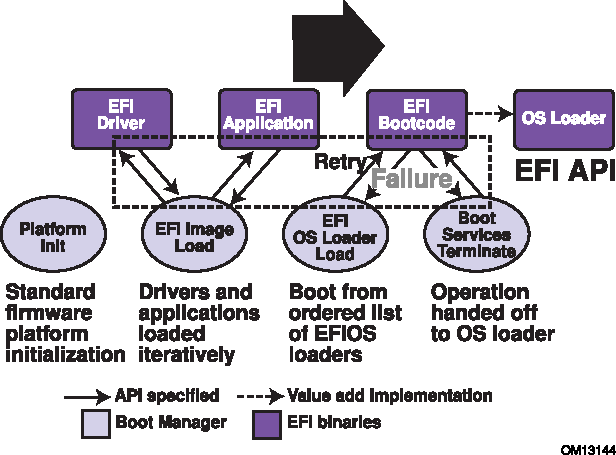
\includegraphics[width=0.9\textwidth]{uefi/uefi_boot_sequence}%
    \caption[\acs{UEFI} Boot Sequence]{\acs{UEFI} Boot Sequence (taken from \cite[Figure 2-1]{uefi-spec})}%
    \label{fig:uefi-boot-sequence}%
\end{figure}
